\chapter{Instalar la librería}\label{cap:instalacion}

En este capítulo se instala \lib\ en un proyecto de TIA Portal. Es la parte más corta: unos diez minutos. Lo que se hace después (adaptar tu código) está en el capítulo~\ref{cap:migracion}.

\section{Qué necesitas}
\begin{itemize}
\item \textbf{TIA Portal V20.} El archivo de la librería (\texttt{CPLabCore\_v\vlib.zal20}) está hecho con V20. Una versión más nueva de TIA abre archivos de versiones anteriores, pero no al revés.
\item \textbf{El archivo} \texttt{CPLabCore\_v\vlib.zal20}, que te pasa quien mantiene la librería.
\item Un \textbf{proyecto con la CPU de tu estación} y su hardware configurado, con los módulos de la CP-Lab (ET\,200SP con dos tarjetas de entradas, dos de salidas y el módulo maestro IO-Link). Si quieres empezar de cero, el capítulo~\ref{cap:migracion} lo cuenta en el camino A.
\end{itemize}

\section{Paso 1: abrir (desarchivar) la librería}\label{sec:abrir-libreria}
Una librería archivada es un archivo comprimido, con extensión \texttt{.zal20}. Hay que \emph{desarchivarla} (extraerla a una carpeta) antes de usarla.

\reiniciapaso
\paso{Abre el panel de librerías}
En el lado derecho de la ventana de TIA, la pestaña vertical \menu{Libraries} (Librerías) despliega el panel. Dentro, la sección \menu{Global libraries} (Librerías globales) tiene una barra de botones; el segundo, \menu{Open global library} (Abrir librería global), abre un cuadro de selección de archivo.

\paso{Elige el tipo «Compressed libraries»}
Por defecto, el cuadro filtra por \menu{Global library}, que son las librerías ya extraídas. Despliega la lista \menu{Tipo} (abajo) y elige \menu{Compressed libraries (*.zal20; ...)}, que es el tipo de los archivos comprimidos. Busca tu archivo \texttt{CPLabCore\_v\vlib.zal20} y ábrelo.

\begin{figure}[ht]
\centering
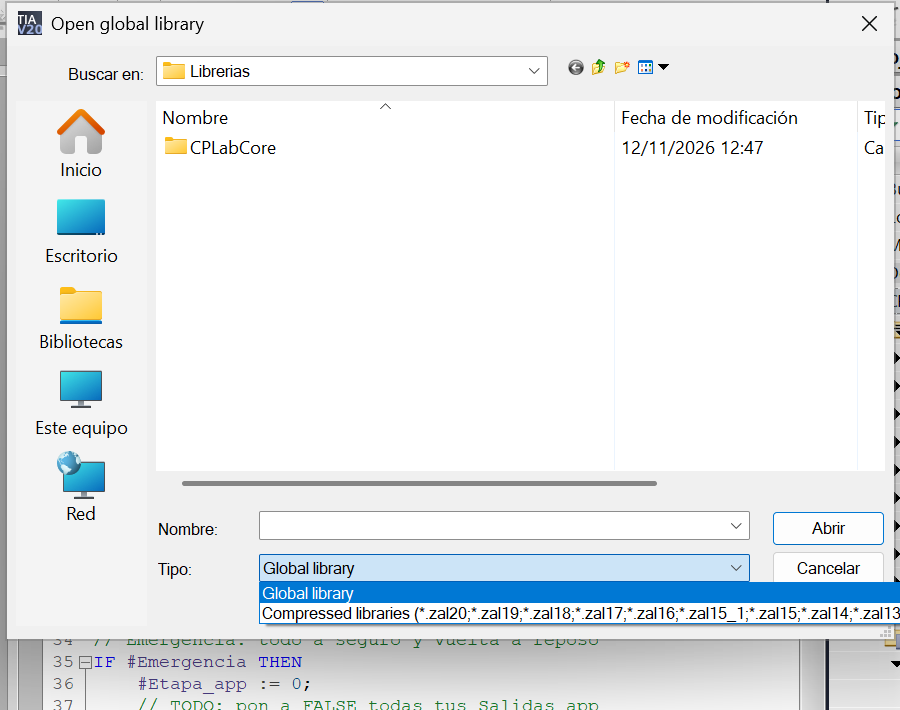
\includegraphics[width=0.78\textwidth]{capturas/abrir_libreria.png}
\caption{El cuadro «Open global library», con la lista de tipos desplegada. El segundo tipo (\textit{Compressed libraries}) es el que hay que elegir para abrir un \texttt{.zal20}.}
\end{figure}

\paso{Elige una carpeta para extraerla}
TIA te pedirá una carpeta donde extraer la librería. Elige una carpeta \textbf{propia y vacía} (por ejemplo, \ruta{C:\textbackslash Librerias\textbackslash CPLabCore}); no la pongas dentro de la carpeta de tu proyecto.

\begin{ojo}
El manual de la CP-Lab explica lo mismo para otra librería con otro nombre de menú: clic derecho en «Librerías globales» y \menu{Desarchivar librería} (en inglés, \textit{Retrieve library}). Según la versión de TIA, el comando está en el botón de abrir o en ese menú contextual. Los dos hacen lo mismo.
\end{ojo}

\comprobar{En la sección \menu{Global libraries} aparece la librería \menu{CPLabCore}. Al desplegarla ves las carpetas \menu{Types} y \menu{Master copies}, como en la figura~\ref{fig:biblioteca}.}

\begin{figure}[ht]
\centering
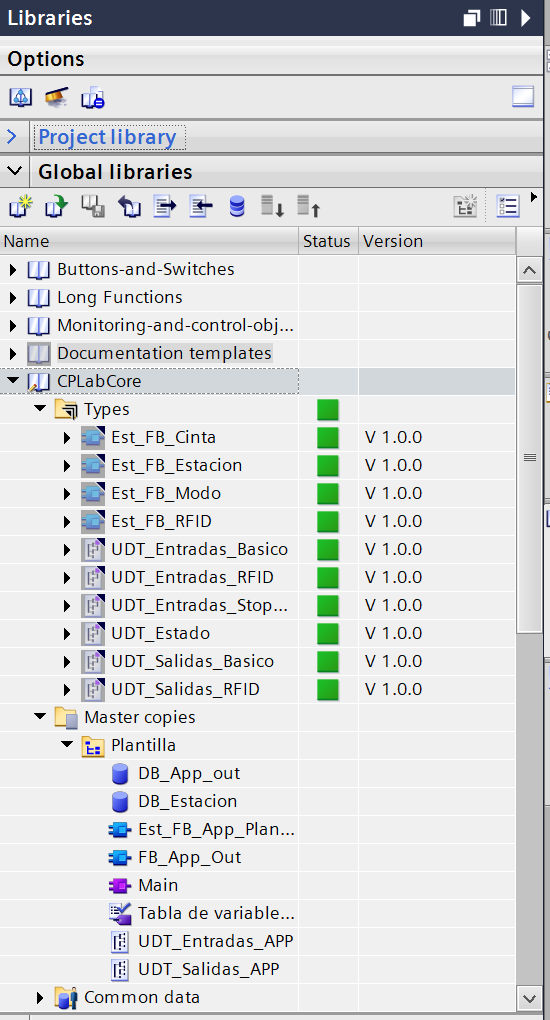
\includegraphics[width=0.62\textwidth]{capturas/biblioteca.png}
\caption{La librería abierta en TIA Portal. En \menu{Types} están los diez tipos, con versión; en \menu{Master copies}, la carpeta \menu{Plantilla}. (Captura de la versión 1.0.0, con el mismo contenido.)}
\label{fig:biblioteca}
\end{figure}

\section{Paso 2: copiar los tipos a tu proyecto}\label{sec:copiar-tipos}
Los tipos se arrastran de la librería al proyecto. Es suficiente arrastrar \textbf{uno}: el bloque \cod{Est\_FB\_Estacion}. TIA añade sola todo lo que necesita.

\paso{Arrastra \cod{Est\_FB\_Estacion}}
En el panel de librerías, abre \menu{CPLabCore $\rightarrow$ Types}. Arrastra \menu{Est\_FB\_Estacion} hasta la carpeta \menu{Program blocks} de tu PLC, en el árbol del proyecto (a la izquierda).

\comprobar{Aparecen en \menu{Program blocks} los cuatro FB (\cod{Est\_FB\_Estacion}, \cod{Est\_FB\_Modo}, \cod{Est\_FB\_Cinta}, \cod{Est\_FB\_RFID}) y en \menu{PLC data types} los seis UDT (\cod{UDT\_Entradas\_Basico}, \cod{UDT\_Entradas\_RFID}, \cod{UDT\_Entradas\_Stopper}, \cod{UDT\_Estado}, \cod{UDT\_Salidas\_Basico} y \cod{UDT\_Salidas\_RFID}).}

\begin{consejo}
Esto se ha comprobado con un proyecto nuevo creado solo para probar la librería: arrastrar \cod{Est\_FB\_Estacion} trajo sus tres FB y sus seis UDT, sin tener que arrastrar ninguno a mano.
\end{consejo}

Los bloques traídos de la librería quedan \textbf{ligados} a ella: en el árbol tienen un icono especial y TIA no deja editarlos desde el proyecto (solo desde la librería). Es lo que se quiere.

\section{Paso 3: copiar la plantilla}\label{sec:copiar-plantilla}
Después se copian de \menu{Master copies $\rightarrow$ Plantilla} las piezas que son tuyas. \textbf{El orden importa} porque unas dependen de otras:

\begin{enumerate}
\item \menu{UDT\_Entradas\_APP} y \menu{UDT\_Salidas\_APP}: los UDT de ejemplo de la aplicación. Solo si los vas a usar como punto de partida; si tu aplicación tiene los suyos, sáltalos.
\item \menu{Tabla de variables estándar}: los siete tags de entradas y salidas (sección~\ref{sec:tags}). Va a \menu{PLC tags}.
\item \menu{DB\_Estacion}: el bloque de datos del contrato.
\item \menu{Est\_FB\_App\_Plantilla}: el esqueleto de aplicación.
\item \menu{Main}: \cod{Main} de ejemplo con las dos llamadas ya cableadas. Si tu proyecto ya tiene un \cod{Main} con tu código, \textbf{no lo sobrescribas todavía}: copia las redes a mano en el capítulo~\ref{cap:migracion}.
\end{enumerate}
Los bloques \menu{FB\_App\_Out} y \menu{DB\_App\_out} son la aplicación completa de la estación Out. Cópialos solo si quieres mirarlos como ejemplo.

\section{Los siete tags de entradas y salidas}\label{sec:tags}
Los tags son lo que enlaza los UDT con los módulos físicos. La copia maestra «Tabla de variables estándar» los trae ya hechos; si prefieres crearlos a mano (por ejemplo, porque tu configuración de hardware es distinta), son estos:

\begin{center}
\small
\begin{tabularx}{\textwidth}{>{\ttfamily}p{3.6cm}>{\ttfamily}p{4.2cm}>{\ttfamily}p{1.9cm}X}
\toprule
\textnormal{\textbf{Nombre}} & \textnormal{\textbf{Tipo de datos}} & \textnormal{\textbf{Dirección}} & \textbf{Módulo} \\
\midrule
Entradas\_APP & UDT\_Entradas\_APP & \%I0.0 & Primer módulo de entradas digitales (tu aplicación). \\
Entradas\_Basico & UDT\_Entradas\_Basico & \%I1.0 & Segundo módulo de entradas (botonera, cinta). \\
Entradas\_Stopper & UDT\_Entradas\_Stopper & \%I42.0 & Dispositivo IO-Link del stopper. \\
Entradas\_RFID & UDT\_Entradas\_RFID & \%I10.0 & Lector RFID por IO-Link. \\
Salidas\_APP & UDT\_Salidas\_APP & \%Q0.0 & Primer módulo de salidas (tu aplicación). \\
Salidas\_Basico & UDT\_Salidas\_Basico & \%Q1.0 & Segundo módulo de salidas (luces, cinta). \\
Salidas\_RFID & UDT\_Salidas\_RFID & \%Q10.0 & Lector RFID por IO-Link. \\
\bottomrule
\end{tabularx}
\end{center}

\begin{ojo}
Son las direcciones de la maqueta real, según el manual de la CP-Lab (apartado 11.2): botonera \cod{\%E1}/\cod{\%A1}, stopper \cod{\%E42}, RFID \cod{\%E10}/\cod{\%A10}, y la aplicación en el primer byte (\cod{\%E0}/\cod{\%A0}). Son \textbf{iguales en todas las estaciones}. Lo único que varía de una estación a otra es el contenido del byte de la aplicación. Si tu proyecto usa otras direcciones (por ejemplo, las del simulador CIROS empiezan en el byte 100), cambia solo la dirección del tag, no el UDT.
\end{ojo}

\section{Paso 4: comprobar que compila}
Compila todo el software del PLC (\menu{Compile $\rightarrow$ Software (rebuild all blocks)}). Qué esperar:

\begin{itemize}
\item \textbf{0 errores} si has copiado la tabla de variables. Es normal un aviso general del estilo «Inputs or outputs are used that do not exist in the configured hardware»: significa que algún tag apunta a una dirección que tu configuración de hardware no tiene todavía. Se resuelve en el capítulo~\ref{cap:migracion}.
\item Si no has copiado los tags, el error es \cod{Tag "Entradas\_Basico" not defined} (y los otros seis). Es exactamente lo que se ve al instalar en un proyecto vacío sin la tabla de variables; no indica ningún problema en la librería.
\end{itemize}

\section{Qué se ha comprobado en la instalación}
Con el archivo de la librería, y desde una instalación aparte (como la haría uno de nosotros), se ha comprobado:
\begin{enumerate}
\item La librería se desarchiva y se abre sin errores.
\item Al arrastrar \cod{Est\_FB\_Estacion} a un proyecto nuevo con una CPU \texttt{1512SP F-1 PN}, aparecen sus tres FB y sus seis UDT.
\item Las copias maestras (los dos UDT de aplicación, \cod{FB\_App\_Out}, \cod{Est\_FB\_App\_Plantilla}, \cod{DB\_App\_out}, \cod{DB\_Estacion} y \cod{Main}) se copian al proyecto.
\item Los tres ejemplos de aplicación (Press, BackCover y Cámara) compilan sin errores en TIA.
\end{enumerate}
La copia de la \emph{tabla de variables} se hace en la interfaz de TIA, arrastrándola. Es la única copia maestra que no se pudo comprobar de forma automática; si no se copiara, la tabla de la sección anterior tiene los siete tags para crearlos a mano.

\section{Actualizar a una versión nueva}
Cuando salga una versión nueva de la librería (capítulo~\ref{cap:mantenimiento}):
\begin{enumerate}
\item Desarchiva el nuevo \texttt{.zal20} como en el paso 1, en una carpeta nueva.
\item En el panel de librerías, haz clic derecho sobre la librería y usa \menu{Update types} (Actualizar tipos): TIA muestra qué tipos de tu proyecto tienen una versión nueva y los actualiza.
\item Vuelve a compilar y repite las pruebas de aceptación (capítulo~\ref{cap:pruebas}).
\end{enumerate}
Como los tipos están ligados a la librería, no pierdes nada tuyo: tus aplicaciones, tu \cod{Main} y tus tags no se tocan.
